% vim: set tabstop=2 softtabstop=2 shiftwidth=2 textwidth=80: %

\documentclass[10pt, compress, xcolor={usenames,dvipsnames}]{beamer}
\usepackage[utf8x]{inputenc}

%%% Theme and style
\usetheme{m}

%%% Packages %%%

% Use T1 and a modern font family for better support of accents, etc.
\usepackage[T1]{fontenc}
\usepackage{palatino}  % Palatino

% Language support
\usepackage[english]{babel}

% Support for easily changing the enumerator in
% enumerate-environments.
\usepackage{enumerate}

% Support for importing images
%\usepackage{graphicx}

% Use hyperlinks
\usepackage{hyperref}

% Don't load xcolors package in beamer: use document class option
% instead...
%\usepackage[usenames,dvipsnames]{xcolor}

% Use colors in tables
%\usepackage[pdftex]{colortbl}

% A nice monospace font for listings, etc.
\usepackage[scaled]{beramono}
%\usepackage{inconsolata}

% Using TikZ for diagrams
\usepackage{tikz}
\usetikzlibrary{shapes,mindmap}
%\usetikzlibrary{er,mindmap,calc,intersections,shapes,arrows,fit,matrix,positioning,decorations.pathmorphing,topaths,trees,automata}
\usepackage{tikz-cd} % for CM-arrow tips.

% Don't use externalize with gradients!!!
%\usetikzlibrary{external,arrows,fit,matrix,positioning}
%\tikzexternalize % Activate externalizing TikZ graphics.

\usepackage{pifont} % for ding
\usepackage[inline]{enumitem}

% Quotes
\usepackage[most]{tcolorbox}

\newtcolorbox{myquote}[1][]{%
  blanker, oversize,%
  left=5pt, %top=1pt, bottom=1pt,%
  borderline west={2pt}{0pt}{mLightBrown},%
  before upper=\indent,%
  parbox=false,%
  #1}


%%% JSON LISTING

\usepackage{listings}

\colorlet{JSONPUNCTCOLOR}{red!60!black}
\definecolor{JSONBACKGROUNDCOLOR}{HTML}{EEEEEE}
\definecolor{JSONDELIMCOLOR}{RGB}{20,105,176}
\colorlet{JSONNUMBERCOLOR}{magenta!60!black}

\lstdefinelanguage{json}{
    captionpos=b,
    basicstyle=\normalfont\ttfamily\small,
    %numbers=left,
    %numberstyle=\scriptsize,
    %stepnumber=1,
    %numbersep=8pt,
    showstringspaces=false,
    breaklines=true,
    frame=none,
    backgroundcolor=\color{JSONBACKGROUNDCOLOR},
    moredelim=**[is][\color{mLightBrown}]{@}{@},
    literate=
     *{0}{{{\color{JSONNUMBERCOLOR}0}}}{1}
      {1}{{{\color{JSONNUMBERCOLOR}1}}}{1}
      {2}{{{\color{JSONNUMBERCOLOR}2}}}{1}
      {3}{{{\color{JSONNUMBERCOLOR}3}}}{1}
      {4}{{{\color{JSONNUMBERCOLOR}4}}}{1}
      {5}{{{\color{JSONNUMBERCOLOR}5}}}{1}
      {6}{{{\color{JSONNUMBERCOLOR}6}}}{1}
      {7}{{{\color{JSONNUMBERCOLOR}7}}}{1}
      {8}{{{\color{JSONNUMBERCOLOR}8}}}{1}
      {9}{{{\color{JSONNUMBERCOLOR}9}}}{1}
      {:}{{{\color{JSONPUNCTCOLOR}{:}}}}{1}
      {,}{{{\color{JSONPUNCTCOLOR}{,}}}}{1}
      {\{}{{{\color{JSONDELIMCOLOR}{\{}}}}{1}
      {\}}{{{\color{JSONDELIMCOLOR}{\}}}}}{1}
      {[}{{{\color{JSONDELIMCOLOR}{[}}}}{1}
      {]}{{{\color{JSONDELIMCOLOR}{]}}}}{1},
}
\lstnewenvironment{lstjson}{\lstset{language=json}}{}

%%% JAVA LISTING

% TODO add colors
\lstnewenvironment{lstjava}{\lstset{language=java, basicstyle=\small}}{}

%%% RUTA LISTING

\definecolor{RUTABACKGROUNDCOLOR}{HTML}{EEEEEE}

\lstdefinelanguage{ruta}{
    captionpos=b,
    basicstyle=\normalfont\ttfamily\small,
    %numbers=left,
    %numberstyle=\scriptsize,
    %stepnumber=1,
    %numbersep=8pt,
    showstringspaces=false,
    breaklines=true,
    frame=single,
    backgroundcolor=\color{RUTABACKGROUNDCOLOR},
}
\lstnewenvironment{lstruta}{\lstset{language=ruta}}{}

%%%% Custom macros %%%%
\newif\ifcompileTreeSlides
%\compileTreeSlidesfalse
\compileTreeSlidestrue

\newcommand{\REST}[1]{{\color{NavyBlue}\ttfamily{#1}}}
\newcommand{\SHELL}[1]{\lstinline[language=bash]!#1!}
\newcommand{\ID}[1]{{\textsc{#1}}}
\newcommand{\SmallArrow}{\ding{228}}
\newcommand{\BigArrow}{$\Longrightarrow$} % TODO find nicer arrow
\newcommand{\hence}{\implies}
\renewcommand{\emph}[1]{\alert{#1}}
\newcommand{\light}{\color{TealBlue}}

% http://tex.stackexchange.com/a/56585/77356
\tikzset{
  invisible/.style={opacity=0},
  visible on/.style={alt=#1{}{invisible}},
  alt/.code args={<#1>#2#3}{%
    \alt<#1>{\pgfkeysalso{#2}}{\pgfkeysalso{#3}} % \pgfkeysalso doesn't change the path
  },
}

%%% Document info %%%

\title{Large-scale Information Extraction from Neuroscientific Literature}

\author{Marco Antognini}

% To show the TOC at the beginning of each section, uncomment this:
% \AtBeginSection[]
% {
%   \begin{frame}<beamer>{Outline}
%     \tableofcontents[currentsection]
%   \end{frame}
% }

% To show the TOC at the beginning of each subsection, uncomment this:
% \AtBeginSubsection[]
% {
%   \begin{frame}<beamer>{Outline}
%     \tableofcontents[currentsection,currentsubsection]
%   \end{frame}
% }


% To uncover everything in a step-wise fashion, uncomment this:
% \beamerdefaultoverlayspecification{<+->}

\setbeamertemplate{footline}[frame number]

\date{%
  \small Spring 2015\\[2em]
  
\includegraphics[height=7mm]{img/epfl-logo}}


%%% Start of the actual document %%%

\begin{document}

\begin{frame}
  \titlepage
\end{frame}

% No outline, too short a talk...
% \begin{frame}{Outline}
%   \tableofcontents
%   % You might wish to add the option [pausesections]
% \end{frame}

\begin{frame}[fragile]{Motivation}

  \begin{myquote}
    The ultimate goal of the \emph{Blue Brain Project} is to reverse engineer
    the mammalian brain.
  \end{myquote}

  \begin{itemize}[label=\SmallArrow]

    \item Interactions between brain regions?

    \item What about effects of specific cells?

    \item And connections with other organs?

    \item \ldots and many many more questions.

  \end{itemize}

  %\vspace{1em}

  The neuroscientific \emph{literature} already holds many answers but\ldots

  %\vspace{1em}
  \pause

  % TODO put this on a new slide.
  \BigArrow \ldots we need a tool to \emph{extract specific information}
  from this colossal amount of text.

\end{frame}

\section{UIMA \& RUTA: in brief}

%\begin{frame}[fragile]{Existing Technologies}

  %\Large

  %\begin{itemize}[label=\textcolor{mLightBrown}{\SmallArrow}, itemsep=4em]

    %\item UIMA engines
      %\pause

    %\item RUTA scripting language

  %\end{itemize}

%\end{frame}

\begin{frame}[fragile]{UIMA}

  \begin{itemize}[label=\SmallArrow, itemsep=1em]

    \item Unstructured Information Management Architecture

    \item \emph{Engines} produce \emph{annotations} (metadata)

    \item Engines are combined to form \emph{pipelines}

    \item Most engines are written in Java

    \item Not limited to neuroscience topics

  \end{itemize}

\end{frame}

\begin{frame}[fragile]{UIMA -- Sentence}

  Assuming we want to find all sentences in this text\ldots

  \vspace{1em}

  \begin{myquote}
    Terminologies which lack semantic connectivity hamper the effective search
    in biomedical fact databases and document retrieval systems. We here focus
    on the integration of two such isolated resources, the term lists from the
    protein fact database UNIPROT and the indexing vocabulary MESH from the
    bibliographic database MEDLINE.
  \end{myquote}

\end{frame}

% TODO: probably not enough time for that...
%\begin{frame}[fragile]{UIMA -- Sentence Pipeline}
%
%  % NOTE: explain what CAS are.
%  % NOTE: mention quickly resources.
%
%  \begin{lstjava}[language=java]
%JCas jCas = UimaTests.getTestCas(text);
%runPipeline(
%  jCas,
%  createEngineDescription(
%    SentenceAnnotator.class,
%    "modelFile", "SentDetectPennBio.bin.gz"
%  )
%  // more engines can come here if needed
%);
%Collection<Sentence> sentences =
%  JCasUtil.select(jCas, Sentence.class);
%  \end{lstjava}
%
%  \pause
%
%  \BigArrow Need to understand Java to write new pipeline even if engines
%  already exist!
%  % NOTE Also Java is not the best tool for every task

%\end{frame}

\begin{frame}[fragile]{UIMA -- Metadata}

  The resulting annotations, presented in JSON format:

  \vspace{1em}

  \begin{lstjson}
"DocumentAnnotation" : [
  { "begin" : 0,    "end" : 328,  "language" : "en" }
],
"Sentence" : [
  { "begin" : 0,    "end" : 135,
    "componentId" :
        "de.julielab.types.OpenNLPSentenceDetector" },
  { "begin" : 136,  "end" : 32
    "componentId" :
        "de.julielab.types.OpenNLPSentenceDetector" }
]
  \end{lstjson}

\end{frame}

\begin{frame}[fragile]{bluima}
  \emph{Bluima} regroups UIMA engines, focusing on neuroscientific engines:

  \begin{itemize}[label=\SmallArrow]

    \item Preprocessing (sentence, tokenizer, PoS, \ldots)

    \item Linnaeus (species recognition)

    \item Oscar (chemistry)

    \item \emph{Brain regions \& their relations}

    \item Proteins

    \item Measures and units

    \item \ldots

  \end{itemize}

\end{frame}

\begin{frame}[fragile]{RUTA}

  \begin{itemize}[label=\SmallArrow, itemsep=1em]

    \item Rule-based Text Annotation

    \item Scripting language

    \item Can \emph{integrate engine} in script

    \item Makes it a bit easier to write UIMA pipeline

  \end{itemize}

\end{frame}

\begin{frame}[fragile]{RUTA -- Simple Script}

  Basic RUTA script tagging dogs as \ID{Animal}:

  \vspace{1em}

  \begin{lstruta}
DECLARE Animal;
W{REGEXP("dog") -> MARK(Animal)};
  \end{lstruta}

\end{frame}

\begin{frame}[fragile]{RUTA -- Part of Speech Pipeline}

  Integration of UIMA engines:

  \vspace{1em}

  \begin{lstruta}
ENGINE SentenceAnnotator;
ENGINE TokenAnnotator;
ENGINE PosTagAnnotator;

Document{-> EXEC(SentenceAnnotator)};
Document{-> EXEC(TokenAnnotator)};
Document{-> EXEC(PosTagAnnotator)};
  \end{lstruta}

  \pause

  \emph{BUT} the engines' settings are stored in an unfriendly XML file\ldots

\end{frame}

\begin{frame}[fragile]{Issues}

  With both raw UIMA and RUTA scripts, some additional issues:

  \vspace{1em}

  \begin{itemize}[label=\SmallArrow, itemsep=1em]

    \item Every user has to go through the hassle of installing UIMA/RUTA
      % tools

    \item Not so trivial to run pipelines

    \item Manage \emph{external resources} (install, update, remove, \ldots)

    \item Manage versions of engines \& pipelines

  \end{itemize}

\end{frame}

\section{Sherlok}

\begin{frame}[fragile]{Sherlok -- Text-Mining Service}

  In a few words:

  \begin{itemize}[label=\SmallArrow, itemsep=1em]

    \item \emph{RESTful} service: 1 server for many users

    \item Based on UIMA $\hence$ existing engines compatible
      \only<2->{{\light(almost)}}

    \item Based on RUTA $\hence$ allowing powerful scripts

    \item Makes it easy to \emph{configure} engines and pipelines

    \item \emph{Automatic resource} management

    \item \emph{Versioning} of pipelines

  \end{itemize}

  \pause

  Sometimes, the Java implementation needs some {\light minor} refactoring.

\end{frame}

\begin{frame}[fragile]{Sherlok -- RESTful}

  What does it mean?

  \vspace{1em}

  Basically, the \emph{HTTP} protocol is all is needed to communicate with Sherlok.

  \vspace{1em}

  \BigArrow \quad Can easily be embedded in any programming language or tool!

  \pause
  {\color{mLightBrown}\hrulefill}

  To annotate some text with the PoS pipeline:

  \REST{GET /annotate/bluima.pos?text=<\ldots>}

\end{frame}

\begin{frame}[fragile]{Sherlok -- Part of Speech Pipeline}

  \begin{center}
    \vspace{-1em}
    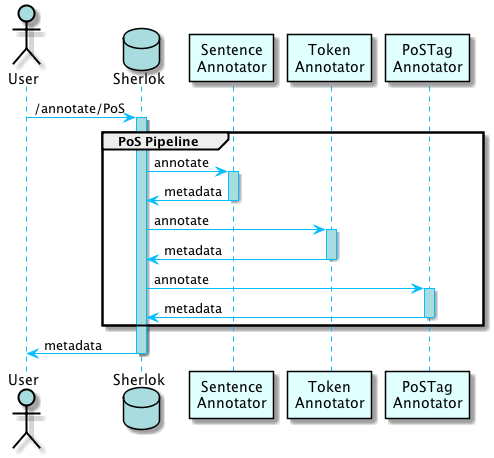
\includegraphics[width=\textwidth, height=0.8\textheight, keepaspectratio]
      {../report/res/sherlok_basic_rest_call.png}
  \end{center}

\end{frame}

\begin{frame}[fragile]{Sherlok -- Running A Pipeline}

  \vspace{-2em}

  \begin{tikzpicture}
    [auto,
     decision/.style={diamond, draw=MidnightBlue, thick, fill=MidnightBlue!20,
                      text width=4.5em, text badly centered,
                      inner sep=1pt},
     action/.style  ={rectangle, draw=black, thick, fill=RoyalBlue!60,
                      text width=5em, text centered, rounded corners,
                      minimum height=4em},
     line/.style    ={draw, thick, ->},
     net/.style     ={draw=JungleGreen, thick, cloud, cloud puffs=9.3,
                      cloud ignores aspect, fill=JungleGreen!20,
                      text width=3em, minimum height=3em},
     actor/.style   ={draw=LimeGreen, thick, circle,fill=LimeGreen!20,
                      minimum height=4em}]

    % Elements
    \matrix [column sep=8mm, row sep=8mm]
    {
      % row 1
      \node [action]      (start)   {start pipeline};     &
      \node [decision]    (cache)   {in cache?};          &
      \node [action]      (jars)    {download jars};      &
      \node [net]         (central) {Internet};           \\
      % row 2
      \node [actor]       (user)    {user};               &
      &
      \node [action, visible on=<2>]
                          (res)     {download resources}; &
      \node [net, visible on=<2>]
                          (web)     {Internet};           \\
      % row 3
      \node [action]      (send)    {send metadata};      &
      \node [action]      (run)     {run RUTA};           &
      \node [action]      (xml)     {generate XML \& RUTA};&
      &                                                   \\
    };

    % Connections
    \begin{scope}[every path/.style=line]
      \path[dashed](user)   --    (start);
      \path       (start)   --    (cache);
      \path       (cache)   --    node [midway] {yes} (run);
      \path       (cache)   --    node [midway] {no} (jars);
      \path[<->]  (jars)    --    (central);
      \path       (xml)     --    (run);
      \path       (run)     --    (send);
      \path[dashed,->|](send)   --    (user);
    \end{scope}

    \only<1>{
      \path[line]   (jars)    --    (xml);
    }

    \only<2>{

      \begin{scope}[every path/.style=line]
        \path[<->]  (res)     --    (web);
        \path       (jars)    --    (res);
        \path       (res)     --    (xml);
      \end{scope}

      % Background rectangle for res + web
      \begin{scope}[on background layer]
        \path[draw=mLightBrown, thick, fill=mLightBrown!10]
          ([xshift=-1em, yshift=1em] res.north west)
          rectangle
          ([xshift=2em, yshift=-1em] res.south west -| web.south east);
      \end{scope}

    }

  \end{tikzpicture}

\end{frame}

\begin{frame}[fragile]{Sherlok -- Kinds of Remote Resource}

  \vspace{-1em}

  \begin{center}

  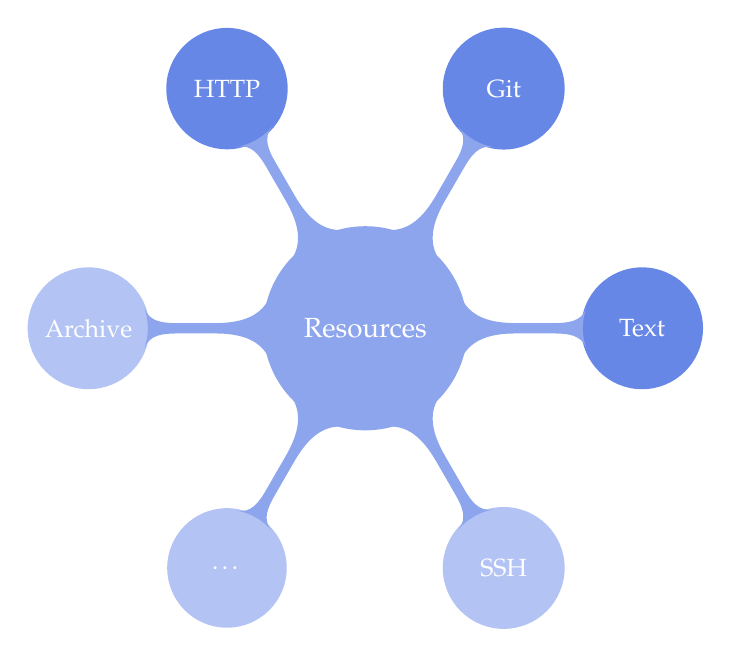
\begin{tikzpicture}
    [auto,
      root concept/.style={concept color=RoyalBlue!60, text=white,
                           minimum size=5em, text width=7em,
                           level distance=2em},
      level 1 concept/.append style={concept, minimum size=2em, text width=4em,
                                     level distance=10em},
      implemented/.style={concept color=RoyalBlue!80},
      todo/.style={concept color=RoyalBlue!40},
    ]

    \path[mindmap]
      node[concept] {Resources}
        [clockwise from=120]
        child { node[concept, implemented] {HTTP} }
        child { node[concept, implemented] {Git} }
        child { node[concept, implemented] {Text} }
        child { node[concept, todo] {SSH} }
        child { node[concept, todo] {\ldots} }
        child { node[concept, todo] {Archive} }
      ;

  \end{tikzpicture}

  \end{center}

\end{frame}

\begin{frame}[fragile]{Sherlok -- Bundle: Engine Configuration}

  \vspace{-1.5em}

  \begin{lstjson}
{
  "name": "bluima.sentence", "version": "1.0.1",
  "dependencies": [
    { "value": "ch.epfl.bbp.nlp:bluima_opennlp:1.0.1" }
  ], "config": {
    @"bluima"@: {
      "type": @"git"@, "ref": "master",
      "url":
        "https://github.com/BlueBrain/bluima_resources.git" }
  }, "engines": [ {
      "name": "SentenceAnnotator",
      "class": "ch.epfl.bbp.uima.ae.SentenceAnnotator",
      "parameters": {
        "modelFile":
          "@$bluima@/opennlp/sentence/SentDetectGenia.bin.gz"
      }
  } ]
}
  \end{lstjson}

\end{frame}

\begin{frame}[fragile]{Sherlok -- Pipeline Configuration}

  \begin{lstjson}
{
  "name": "countries", "version": "1",
  "description": "Example that annotates countries",
  "config": {
    @"countries"@: {
      "type": @"http"@, "mode": "ruta",
      "url": "https://example.com/countries.txt"
    }
  }, "script": [
    "WORDLIST CountriesList = '@$countries@';",
    "DECLARE Country;",
    "Document{-> MARKFAST(Country, CountriesList)};"
  ]
}
  \end{lstjson}

\end{frame}

\plain{\Huge Demo!}
% NOTE: HTML demo with Brain Regions

\begin{frame}{Thank you!}
  \begin{center}
    \Huge Questions?
  \end{center}
  \vspace{2em}
  \begin{center}
    Check it out\vspace{.5em}\\
    {\light\url{http://sherlok.io}}
  \end{center}
\end{frame}

\end{document}
